\documentclass[conference]{IEEEtran}
\IEEEoverridecommandlockouts
\usepackage[T1]{fontenc}
\usepackage{cite}
\usepackage{amsmath,amssymb}
\usepackage{graphicx}
\usepackage{booktabs}
\usepackage{multirow}
\usepackage{tikz}
\usetikzlibrary{arrows.meta,positioning,fit,calc}
\usepackage{pgfplots}
\pgfplotsset{compat=1.18}
\usepackage{xcolor}
\usepackage[hidelinks]{hyperref}
\usepackage{url}
\usepackage{fancyvrb}

\newcommand{\Fp}{F\'{}}  % NASA F Prime
\newcommand{\tool}[1]{\texttt{#1}}

\begin{document}

\title{On-Premises LLM Assistance for Embedded Flight Software:\\
Measured Sizing, Traceability Recovery and Execution-Verified Test Generation}

\author{\IEEEauthorblockN{Djoud El Hak Belkhir}
\IEEEauthorblockA{M2 Data, Knowledge and Hybrid AI\\
Universit\'e Paris-Saclay, France}}

\maketitle

\begin{abstract}
Teams that build embedded radio and flight software often cannot send source code to a hosted model, yet they want
the same assistance for coding, refactoring, documentation and testing. We present an open, fully on-premises
platform that serves open-weight code models, connects them to a team's code, tests, requirements and CI through
the Model Context Protocol (MCP), and sizes the hardware from measurements. We study three questions on NASA's
\Fp{} flight-software framework with two 2025 open-weight models (Qwen3-Coder-30B-A3B, a mixture-of-experts model,
and the dense Devstral-Small-2-24B) served on two Tesla T4 GPUs. (i)~A roofline model calibrated per engine and
architecture class predicts single-stream decode speed within $\pm$11\,\% leave-one-model-out and the chat capacity
of one llama.cpp server within 7\,\%. (ii)~Ranking the 3{,}261 test cases of \Fp{} for each of 151 requirements,
reciprocal-rank fusion of BM25 and dense retrieval inside a module-graph prior recovers requirement-to-test links
with a mean average precision of 0.609, while an LLM reranker lowers it. (iii)~An agent that may write only test
code, and whose tests must pass a policy check, compile and pass before being committed for review, closes
18 of 28 traceability gaps with each model; it closed 11 and 8 before a failure taxonomy pointed to general prompt
and tooling fixes (exact McNemar $p = 0.016$ and $0.013$). Its tests kill 66\,\% and 52\,\% of seeded mutants.
All code, data and notebooks are released.
\end{abstract}

\begin{IEEEkeywords}
large language models, on-premises deployment, capacity planning, requirements traceability, unit test generation,
flight software, Model Context Protocol, mutation testing
\end{IEEEkeywords}

\section{Introduction}
Code assistants built on large language models (LLMs) are now common in software teams, but the default
deployment, a hosted model that receives the code, is ruled out for many embedded and defence projects by export
control, contractual or security constraints. Open-weight code models make on-premises use possible. Three
practical questions then decide whether such a deployment is worth it, and they are rarely answered together.
\emph{How much hardware} does a team need, given that vendor peak numbers do not predict engine behaviour?
\emph{How is the model grounded} in the team's own artefacts (requirements, tests, design documents) rather than
in its training data? And \emph{how can its output be trusted} in a domain where a plausible but wrong test is
worse than no test?

We answer them on a single, reproducible case: NASA's open-source \Fp{} framework~\cite{bocchino2018fprime}
(v4.4.1), whose design documents define requirements and whose unit tests cite them with
\tool{REQUIREMENT("ID")} tags. Our contributions are:
\begin{itemize}
\item an open on-premises platform (Fig.~\ref{fig:arch}): engine-agnostic model serving, a typed knowledge graph of
  code, tests, requirements and documents exposed through an MCP server~\cite{mcp2025}, CI access through
  Jenkins' MCP plugin, and an air-gap smoke test run in CI;
\item a sizing method that calibrates a roofline model~\cite{williams2009roofline} separately for dense and
  mixture-of-experts (MoE) models and for each engine, validated leave-one-model-out and against load tests;
\item a traceability-recovery benchmark on \Fp{} (151 requirements $\times$ 3{,}261 tests, tags masked) comparing
  lexical, dense, graph-constrained and LLM-reranked retrieval with bootstrap confidence intervals;
\item a bounded-authority test-generation agent whose every output is gated by build, test and policy checks,
  and a taxonomy of its 121 failed attempts that pointed to general fixes and a significant improvement.
\end{itemize}

\section{Related Work}
\emph{LLM-based unit test generation.} Sch\"afer et al.~\cite{schafer2024testpilot} generate JavaScript tests from
API documentation and repair failing ones; CodaMosa~\cite{lemieux2023codamosa} uses an LLM to escape coverage
plateaus of search-based testing~\cite{fraser2011evosuite}; Meta's TestGen-LLM~\cite{alshahwan2024meta} keeps a
generated test only if it builds, passes reliably and increases coverage, a filtering principle we adopt and extend
with mutation analysis~\cite{jia2011mutation} and requirement tags. Agentic systems such as
SWE-agent~\cite{yang2024sweagent} act on repositories through tool interfaces; our agent instead restricts the
model to test code and keeps every other action deterministic. Public benchmarks (HumanEval~\cite{chen2021codex},
SWE-bench~\cite{jimenez2024swebench}) are Python-centred and exposed to training-set contamination, which motivates
the small, execution-scored embedded C suite of Section~\ref{sec:eval}.

\emph{Traceability recovery.} Information-retrieval approaches to trace links date back to Antoniol et
al.~\cite{antoniol2002traceability} and are surveyed by Borg et al.~\cite{borg2014traceability}; LLM prompting for
trace links was studied by Rodriguez et al.~\cite{rodriguez2023prompts}. We combine BM25~\cite{robertson2009bm25},
dense embeddings~\cite{zhang2025qwen3embedding} and reciprocal-rank fusion~\cite{cormack2009rrf} with a prior from
the module graph, and use the retrieval both as a benchmark and as the context source of a retrieval-augmented
agent~\cite{lewis2020rag}.

\emph{Serving and sizing.} vLLM~\cite{kwon2023vllm} batches requests with paged KV-cache memory; llama.cpp~\cite{llamacpp}
runs quantized GGUF models on modest GPUs. Quantization (e.g., AWQ~\cite{lin2024awq}) and attention kernels
(FlashAttention-2~\cite{dao2024flashattention2}) change achievable throughput by GPU generation, which is why we
calibrate on measurements rather than on datasheets.

\section{Platform}
\begin{figure}[t]
\centering
% Fig. 1 -- platform architecture (TikZ). Included by main.tex.
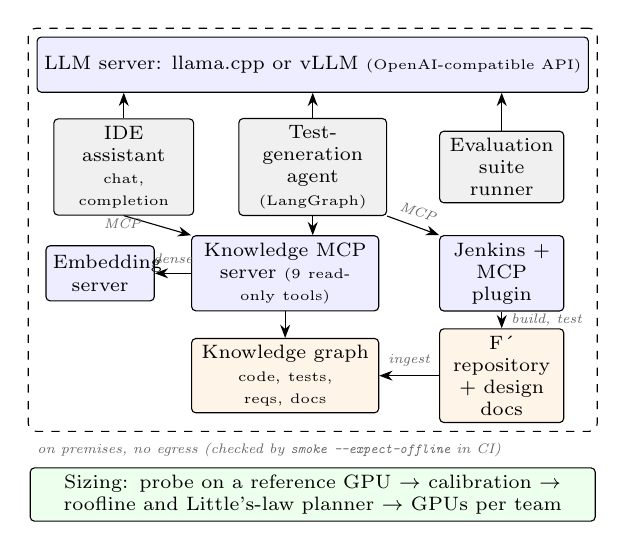
\begin{tikzpicture}[
  font=\scriptsize, >=Stealth,
  box/.style={draw, rounded corners=1.5pt, align=center, inner sep=2.5pt, minimum height=7mm, fill=white},
  client/.style={box, fill=black!6},
  svc/.style={box, fill=blue!7},
  data/.style={box, fill=orange!9},
  lab/.style={font=\tiny\itshape, text=black!60},
]
% model serving (top)
\node[svc, minimum width=61mm] (llm) at (2.4,0) {LLM server: llama.cpp or vLLM {\tiny(OpenAI-compatible API)}};
% clients (middle)
\node[client, text width=16mm] (ide) at (0,-1.3) {IDE assistant\\{\tiny chat, completion}};
\node[client, text width=17mm] (agent) at (2.4,-1.3) {Test-generation\\agent {\tiny(LangGraph)}};
\node[client, text width=14mm] (eval) at (4.8,-1.3) {Evaluation\\suite runner};
% MCP servers and embeddings
\node[svc, text width=12mm] (emb) at (-0.3,-2.65) {Embedding\\server};
\node[svc, text width=22mm] (kmcp) at (2.05,-2.65) {Knowledge MCP\\server {\tiny(9 read-only tools)}};
\node[svc, text width=14mm] (ci) at (4.8,-2.65) {Jenkins +\\MCP plugin};
% data
\node[data, text width=22mm] (kg) at (2.05,-3.95) {Knowledge graph\\{\tiny code, tests, reqs, docs}};
\node[data, text width=14mm] (repo) at (4.8,-3.95) {F\'{} repository\\+ design docs};
% edges
\foreach \c in {ide, agent, eval} \draw[->] (\c.north) -- (\c.north |- llm.south);
\draw[->] (ide.south) -- node[lab, left, pos=0.4]{MCP} (kmcp.north west);
\draw[->] (agent.south) -- (agent.south |- kmcp.north);
\draw[->] (agent.south east) -- node[lab, above, sloped]{MCP} (ci.north west);
\draw[->] (kmcp) -- (kg);
\draw[->] (kmcp) -- node[lab, above]{dense} (emb);
\draw[->] (repo) -- node[lab, above]{ingest} (kg);
\draw[->] (ci) -- node[lab, right]{build, test} (repo);
% boundary
\node[draw, dashed, rounded corners=3pt, inner sep=3pt, fit=(llm)(emb)(kg)(repo)(eval),
  label={[lab, anchor=north west, yshift=-0.5pt]south west:on premises, no egress (checked by \texttt{smoke -{}-expect-offline} in CI)}] (bnd) {};
% sizing pipeline
\node[box, fill=green!7, text width=70mm, minimum height=5.5mm, below=4.5mm of bnd.south] (siz)
  {Sizing: probe on a reference GPU $\rightarrow$ calibration $\rightarrow$ roofline and Little's-law planner $\rightarrow$ GPUs per team};
\end{tikzpicture}

\caption{Platform architecture. Clients reach models through an OpenAI-compatible API and engineering knowledge
through MCP; the knowledge server's dense search calls the local embedding server. Everything runs inside the
site boundary; sizing is an offline pipeline.}
\label{fig:arch}
\end{figure}

\emph{Knowledge graph.} An ingester parses \Fp{} with tree-sitter and the design documents' requirement tables
into a typed graph: 1{,}250 files (206{,}656 lines of code), 5{,}499 functions, 3{,}261 test cases, 560
requirements from 83 documents, 21{,}681 resolved call edges (including the \Fp{} autocoder conventions, e.g.\ a
test calling \tool{sendCmd\_X} exercises \tool{X\_cmdHandler}) and 481 \textsc{verifies} edges taken only from
explicit tags. Identifiers derive from source locations, so the same commit always yields a byte-identical
snapshot; it builds in about 3\,s on a laptop CPU. The graph doubles as an audit: 288 requirements specified as
verified by test have no tagged test, 12 cited IDs are defined nowhere and 12 are cited by another component's
tests.

\emph{MCP server.} Nine read-only tools serve IDE assistants and the agent alike: text and semantic search,
symbol lookup, callers and callees, requirement lookup and tracing (\tool{trace\_requirement} ranks candidate
tests and related code), coverage gaps per module, and module listings and overviews. They run over stdio or HTTP,
from an in-memory snapshot or Neo4j.

\emph{Deployment.} Container profiles cover CPU, single-GPU llama.cpp and multi-GPU vLLM. Model servers require API
keys and bind to localhost; an offline overlay moves all services to an internal network and runs a smoke test
that fails if any outbound connection succeeds, on every CI run.

\section{Sizing Model}\label{sec:sizing}
Memory is the weight size (measured artefact, or parameters $\times$ bits per weight) plus, per sequence, the KV
cache $2\,L_{\mathrm{attn}} H_{kv} d_h b\,n$ for $n$ tokens (and recurrent state for linear-attention layers).
Decode is bandwidth bound: a step at batch $B$ reads the touched weights and every sequence's cache,
\begin{equation}
t_{\mathrm{dec}}(B) = \frac{W_{\mathrm{dense}} + W_{\mathrm{exp}}\bigl(1-(1-k/E)^{B}\bigr) + B\,c\,s_{kv}}
{\eta_{d}\,\beta\,g},
\label{eq:decode}
\end{equation}
where an MoE layer routes each token to $k$ of $E$ experts, $c$ is the average context, $s_{kv}$ the cache bytes
per token, $\beta$ the peak bandwidth and $g$ the tensor-parallel scale (1 for llama.cpp's layer split, whose GPUs
work in sequence). Prefill is compute bound at $2P_{\mathrm{act}}$ FLOPs per token plus attention, at a fraction
$\eta_p$ of peak FP16. The efficiencies $\eta_d, \eta_p$ are the only fitted parameters, estimated per engine and
separately for dense and MoE models because a single shared value mispredicted MoE prefill by up to $+239\,\%$. Capacity then
follows from Little's law~\cite{little1961}: with request classes of rate $\lambda_i$ and service time $T_i$, the
concurrent sequences $C=\sum_i \lambda_i T_i$ must fit in $B^{*}$, the largest batch whose per-sequence decode speed
meets the service-level objective (SLO), after the replica's prefill time $U$ is deducted:
$R \ge h\,(C/B^{*} + U)$ replicas for headroom $h$.

\section{Experimental Setup}
All GPU measurements ran in Kaggle batch notebooks on two NVIDIA Tesla T4 GPUs (16\,GB, Turing, SM~7.5).
We compare Qwen3-Coder-30B-A3B-Instruct~\cite{yang2025qwen3} (MoE, 30.5\,B parameters, 3.3\,B active, 8 of 128
experts) and Devstral-Small-2-24B~\cite{mistral2025devstral2} (dense, 24.0\,B), both released in 2025 under
Apache~2.0. Both run on llama.cpp (build b11953, Q4\_K\_M weights, layer split, 4 slots of 16k tokens); Qwen3-Coder
also runs on vLLM~0.32 (AWQ, tensor parallel~2). A probe run measured five models; benchmark run~2 (3.4\,h)
produced the traceability, evaluation and agent-v1 results and run~3 (2.8\,h) the serving sweeps and agent~v2.
Table~\ref{tab:probe} gives the single-stream baseline. On this bandwidth-bound GPU the MoE model decodes about
five times faster than the dense one, and vLLM's AWQ prefill (no Marlin kernels, no FlashAttention-2 on SM~7.5) is
five times slower than llama.cpp's.

\begin{table}[t]
\caption{Probe on 2$\times$T4, 4-bit weights, single stream}
\label{tab:probe}
\centering
\footnotesize
\setlength{\tabcolsep}{3.2pt}
\begin{tabular}{@{}llrrr@{}}
\toprule
Model & Engine & Decode & Prefill & 4 streams \\
 & & tok/s & tok/s & tok/s \\
\midrule
Qwen3-Coder-30B-A3B (MoE) & llama.cpp & 81.9 & 1{,}445 & 151 \\
Qwen3-Coder-30B-A3B (MoE) & vLLM AWQ & 101.0 & 283 & 245 \\
Qwen3.6-35B-A3B (MoE) & llama.cpp & 60.9 & 1{,}326 & 107 \\
Devstral-Small-2-24B (dense) & llama.cpp & 15.9 & 649 & 28 \\
Qwen3.8-27B (dense) & llama.cpp & 13.9 & 550 & 29 \\
\bottomrule
\end{tabular}
\end{table}

\section{Results}
\subsection{Serving capacity and sizing accuracy}
Fig.~\ref{fig:serving} shows the IDE-chat profile (about 2.5k-token prompts, 400-token answers); every concurrency
level uses new prompts so that no level is served from a cache warmed by the previous one. At a 20\,tok/s per-user
SLO, one 2$\times$T4 server holds about four concurrent chat users with either engine. llama.cpp stops scaling at
its four slots: past them, requests queue and the median time to first token grows from 5.7\,s to 71\,s at 16
streams. vLLM keeps batching (98\,tok/s total at 16 streams) at 7\,tok/s per user. The ranking flips for agent
steps (about 9k-token prompts with a shared prefix): llama.cpp serves 0.29--0.44 requests/s against 0.10--0.14 for
vLLM, whose long-prompt prefill is the bottleneck on Turing. Devstral stays below the SLO even alone (15\,tok/s).

\begin{figure}[t]
\centering
% Fig. 3 -- per-user decode speed vs concurrency, chat profile, benchmark run 3 (data: serving_chat.dat).
\begin{tikzpicture}
\begin{axis}[
  width=\columnwidth, height=44mm,
  xmode=log, log basis x=2, xtick={1,2,4,8,16}, xticklabels={1,2,4,8,16},
  xlabel={concurrent streams}, ylabel={tok/s per user},
  ymin=0, ymax=80, ytick={0,20,40,60,80},
  grid=major, grid style={black!10},
  tick label style={font=\scriptsize}, label style={font=\scriptsize},
  legend style={font=\tiny, at={(0.98,0.98)}, anchor=north east, draw=none, fill=white, fill opacity=0.85, text opacity=1, row sep=-1pt},
  every axis plot/.append style={thick, mark size=1.6pt},
  xmin=0.85, xmax=19,
]
\addplot[color=blue!75!black, mark=*] table[x=streams, y=qwenllama] {figures/serving_chat.dat};
\addlegendentry{Qwen3-Coder, llama.cpp}
\addplot[color=teal!80!black, mark=square*] table[x=streams, y=qwenvllm] {figures/serving_chat.dat};
\addlegendentry{Qwen3-Coder, vLLM}
\addplot[color=orange!85!black, mark=triangle*] table[x=streams, y=devllama] {figures/serving_chat.dat};
\addlegendentry{Devstral, llama.cpp}
\addplot[black!60, dashed, thin, mark=none, domain=0.85:19] {20};
\addlegendentry{20 tok/s SLO}
\end{axis}
\end{tikzpicture}

\caption{Decode speed each user sees in the chat profile (median), benchmark run~3. The dashed line is the
20\,tok/s SLO used for sizing.}
\label{fig:serving}
\end{figure}

Table~\ref{tab:sizing} validates the sizing model. Fitted on the probe, the llama.cpp efficiencies are
$\eta_d = 0.771 / 0.590$ and $\eta_p = 0.508 / 0.202$ (dense / MoE); vLLM reaches $\eta_d = 0.374$ and
$\eta_p = 0.030$ on this GPU. Decode is predicted within $\pm 11\,\%$ leave-one-model-out and within 4\,\% on run~3,
whose contexts the calibration never saw. MoE prefill is not predictable from one other MoE model with a different
attention design (Qwen3.6 has linear-attention layers). The planner's chat capacity for one llama.cpp server is
within 7\,\% of the load test; on vLLM it is conservative by half, because its prefill efficiency was fitted on a
13k-token prompt and Turing prefill is much slower on long prompts. Applied to larger GPUs, the same planner gives,
for 100 engineers using chat and agents, 6 L4 or 2 L40S or 1 H100 for Qwen3-Coder; such tables hold only to first
order until the probe is re-run on the candidate GPU, which the tooling is designed for.

\begin{table}[t]
\caption{Sizing model validation (llama.cpp unless noted)}
\label{tab:sizing}
\centering
\footnotesize
\setlength{\tabcolsep}{3pt}
\begin{tabular}{@{}lrrr@{}}
\toprule
Prediction & Measured & Predicted & Error \\
\midrule
\multicolumn{4}{@{}l}{\emph{Leave-one-model-out, decode tok/s}} \\
\quad Qwen3.8-27B (dense) & 13.9 & 13.7 & $-1.5\,\%$ \\
\quad Devstral-Small-2-24B (dense) & 15.9 & 16.1 & $+1.5\,\%$ \\
\quad Qwen3-Coder-30B-A3B (MoE) & 81.9 & 90.6 & $+10.6\,\%$ \\
\quad Qwen3.6-35B-A3B (MoE) & 60.9 & 55.1 & $-9.6\,\%$ \\
\multicolumn{4}{@{}l}{\emph{Independent run 3, decode tok/s at 2.8k context}} \\
\quad Qwen3-Coder & 73.6 & 76.7 & $+4\,\%$ \\
\quad Devstral & 15.2 & 15.6 & $+3\,\%$ \\
\multicolumn{4}{@{}l}{\emph{Chat capacity, requests/s at 20 tok/s per user}} \\
\quad Qwen3-Coder, llama.cpp & 0.174 & 0.187 & $+7\,\%$ \\
\quad Qwen3-Coder, vLLM & 0.185 & 0.090 & $-51\,\%$ \\
\bottomrule
\end{tabular}
\end{table}

\subsection{Requirement-to-test traceability recovery}
The 481 tags link 151 requirements to their tests. We mask tags and IDs and let each method rank all 3{,}261 test
cases for every requirement; ties are broken randomly and averaged. Dense retrieval uses Qwen3-Embedding-0.6B with
task instructions. The graph prior ranks tests of the requirement's module first, then tests that call into it.
Table~\ref{tab:trace} reports means with 95\,\% bootstrap intervals~\cite{efron1993bootstrap}. Lexical and dense
retrieval are equally good alone but fail on different requirements: their fusion inside the graph prior is best
(MAP 0.609), $+0.04$ over graph-constrained BM25. Pointwise LLM reranking of the top ten lowers precision at the
top (Recall@1 from 0.350 to 0.297): the judge scores pairs without the module context and produces many ties, at a
cost of ten model calls per requirement.

\begin{table}[t]
\caption{Traceability recovery on \Fp{} (151 requirements, 3{,}261 candidates)}
\label{tab:trace}
\centering
\footnotesize
\setlength{\tabcolsep}{3pt}
\begin{tabular}{@{}lccc@{}}
\toprule
Method & MAP [95\,\% CI] & R@1 & R@10 \\
\midrule
Graph prior only & 0.249 [0.220, 0.278] & 0.073 & 0.550 \\
Dense (Qwen3-Embedding-0.6B) & 0.479 [0.428, 0.531] & 0.261 & 0.713 \\
BM25 & 0.488 [0.427, 0.548] & 0.297 & 0.677 \\
Graph + BM25 & 0.569 [0.513, 0.626] & 0.330 & 0.781 \\
Graph + dense & 0.573 [0.521, 0.619] & 0.303 & 0.817 \\
\textbf{Graph + RRF(BM25, dense)} & \textbf{0.609 [0.553, 0.660]} & \textbf{0.350} & \textbf{0.821} \\
\quad + LLM rerank of top 10 & 0.584 [0.535, 0.633] & 0.297 & 0.822 \\
\bottomrule
\end{tabular}
\end{table}

\subsection{Embedded C evaluation suite}\label{sec:eval}
To choose a model for the assistant use cases we wrote 27 C99 tasks in the style of radio and flight software
(CCSDS headers, COBS framing, CRCs, Hamming and convolutional codes, Q15 arithmetic, wrap-around-safe timers) in
four categories, all scored by execution: \emph{generate} (hidden tests under \tool{-Wall -Wextra -Wpedantic}, no
heap or stdio), \emph{test generation} (the tests must pass on the correct implementation and fail on every one of
4--6 seeded mutants), \emph{refactor} (tests still pass and maximum cyclomatic complexity strictly decreases) and
\emph{document} (code tokens unchanged and complete Doxygen tags). The suite validates itself: references pass,
generated stubs fail, reference tests kill every mutant, and prompts never contain hidden material.
Table~\ref{tab:eval} gives one sample per task at temperature 0.2. Qwen3-Coder passes 15 tasks against 10, with a
four times lower median latency; on the same tasks 7 are passed only by Qwen3-Coder and 2 only by Devstral (exact
McNemar~\cite{mcnemar1947} $p = 0.18$), a direction rather than a significant difference. Re-scoring every failure
from the stored outputs shows the failures are the models': 8 of 12 generated test programs fail on the
\emph{correct} implementation because hand-computed expected values are wrong, both models mishandle stated
bit-level conventions (COBS blocks, Hamming bit layout), and failed refactorings change behaviour.

\begin{table}[t]
\caption{Embedded C suite: tasks passed (one sample, pass@1)}
\label{tab:eval}
\centering
\footnotesize
\setlength{\tabcolsep}{3.2pt}
\begin{tabular}{@{}lcccccc@{}}
\toprule
Model & Gen. & Tests & Refact. & Doc. & Total & Median \\
 & /12 & /6 & /5 & /4 & /27 & latency \\
\midrule
Qwen3-Coder & \textbf{9} & 0 & 2 & \textbf{4} & \textbf{15} & \textbf{21\,s} \\
Devstral & 5 & 1 & 2 & 2 & 10 & 85\,s \\
\bottomrule
\end{tabular}
\end{table}

\subsection{Test generation for traceability gaps}
\emph{Agent design.} The agent (Fig.~\ref{fig:agent}) is a LangGraph~\cite{langgraph} state machine. The model
writes only new \tool{Tester} methods and \tool{TEST()} cases in two fenced blocks; declarations, insertion points
and includes are derived by a patcher. Before building, a policy rejects changes outside the component's three test
files, reused names, missing assertions, unsafe calls (\tool{system}, \tool{fork}, threads, inline assembly) and
any requirement tag other than the target's. A test is accepted only if the \Fp{} unit tests build with
\tool{-Werror}, the new test passes three runs (\Fp{} tests use random seeds) and the full suite still passes; it
is then committed on a review branch with an AI-use disclosure, as \Fp{}'s contribution policy asks. Context is
deterministic and budgeted at 32{,}000 characters, so that a 16k-token slot holds the task, one previous answer,
its diagnostics and the new answer. Repairs (at most three attempts) receive condensed compiler errors with
did-you-mean hints, test output, and for \Fp{} assertions the asserted source line. Fault detection is measured
after the fact, never shown to the model: the new test alone runs against up to four mutants of the lines it
executes (inverted conditions, swapped success statuses, deleted port calls).

\begin{figure}[t]
\centering
% Fig. 3 -- the agent's state graph (TikZ). Included by main.tex.
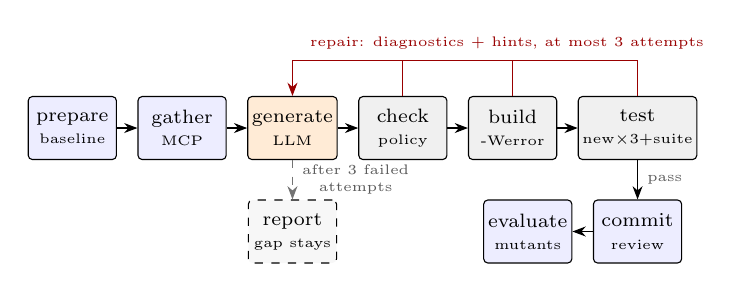
\begin{tikzpicture}[
  font=\scriptsize, >=Stealth, node distance=2.6mm,
  n/.style={draw, rounded corners=1.5pt, align=center, inner sep=1.5pt, minimum height=8mm, minimum width=11.2mm, fill=blue!7},
  llm/.style={n, fill=orange!16},
  gate/.style={n, fill=black!6},
  lab/.style={font=\tiny, text=black!65, align=center},
]
\node[n] (prep) {prepare\\{\tiny baseline}};
\node[n, right=of prep] (gath) {gather\\{\tiny MCP}};
\node[llm, right=of gath] (gen) {generate\\{\tiny LLM}};
\node[gate, right=of gen] (chk) {check\\{\tiny policy}};
\node[gate, right=of chk] (bld) {build\\{\tiny -Werror}};
\node[gate, right=of bld] (tst) {test\\{\tiny new$\times$3+suite}};
\node[n, below=5mm of tst] (com) {commit\\{\tiny review}};
\node[n, left=of com] (evl) {evaluate\\{\tiny mutants}};
\node[n, below=5mm of gen, fill=black!3, dashed] (fin) {report\\{\tiny gap stays}};
\foreach \a/\b in {prep/gath, gath/gen, gen/chk, chk/bld, bld/tst} \draw[->] (\a) -- (\b);
\draw[->] (tst) -- node[lab, right]{pass} (com);
\draw[->] (com) -- (evl);
% repair bus above the row
\coordinate (bus) at ($(gen.north)+(0,4.5mm)$);
\draw[->, red!60!black] (chk.north) -- (chk.north |- bus) -- (bus) -- (gen.north);
\draw[red!60!black] (bld.north) -- (bld.north |- bus) -- (chk.north |- bus);
\draw[red!60!black] (tst.north) -- (tst.north |- bus) -- (bld.north |- bus);
\node[lab, above=0.2mm of bus, anchor=south west, xshift=1mm, text=red!60!black]
  {repair: diagnostics + hints, at most 3 attempts};
\draw[->, dashed, black!55] (gen.south) -- node[lab, right]{after 3 failed\\attempts} (fin.north);
\end{tikzpicture}

\caption{The agent's graph. Only \emph{generate} calls the LLM; every other node is deterministic and takes its
arguments from the requirement, never from model output. Red edges are repairs; the dashed edge ends the run without a commit.}
\label{fig:agent}
\end{figure}

\emph{Targets.} We select the 28 gaps of four components (\tool{Svc/ComStub}, \tool{Svc/ComRetry},
\tool{Svc/PrmDb}, \tool{Svc/FprimeRouter}) that have the standard test harness, build and pass at baseline, and
show no ID mismatch in the audit.

\emph{From v1 to v2.} We classify every failed attempt by its first matching diagnostic rule (Fig.~\ref{fig:causes}).
In v1, 65 of 121 failed attempts were dispatch calls on the wrong object or on passive components: the prompt
described the active-component dispatch rule without stating which kind the component under test was (three of
four are passive), and the did-you-mean hints offered a function that \Fp{}~v4 no longer has. Eight more came from
a patcher bug on namespace-qualified definitions. Agent v2 states the component kind and its exact dispatch call
in the task, fixes the patcher, reuses a code block that a repair answer leaves out, adds the asserted line to
assertion failures and lists the \tool{-Werror} rules. These are general rules, not per-requirement fixes. Both
causes fell to zero (Fig.~\ref{fig:causes}).

\begin{figure}[t]
\centering
% Fig. 4 -- failed attempts by primary cause, agent v1 (run 2) vs v2 (run 3) (data: failure_causes.dat).
\begin{tikzpicture}
\begin{axis}[
  xbar stacked, bar width=7pt,
  width=0.96\columnwidth, height=40mm,
  xmin=0, xmax=70, xlabel={failed attempts (28 requirements, $\le$3 attempts each)},
  symbolic y coords={{Devstral v2},{Devstral v1},{Qwen v2},{Qwen v1}}, ytick=data,
  y dir=normal, enlarge y limits=0.2,
  tick label style={font=\scriptsize}, label style={font=\scriptsize},
  legend style={font=\tiny, at={(0.5,1.03)}, anchor=south, legend columns=3, draw=none, column sep=2pt},
  grid=major, ymajorgrids=false, grid style={black!10},
  every axis plot/.append style={draw=white, line width=0.3pt},
]
\addplot[fill=red!65!black] table[y=run, x=dispatch] {figures/failure_causes.dat};
\addlegendentry{wrong dispatch call}
\addplot[fill=red!35] table[y=run, x=qualified] {figures/failure_causes.dat};
\addlegendentry{qualified definition (agent bug)}
\addplot[fill=orange!75!black] table[y=run, x=compile] {figures/failure_causes.dat};
\addlegendentry{other compile error}
\addplot[fill=yellow!70!orange] table[y=run, x=policy] {figures/failure_causes.dat};
\addlegendentry{policy rejection}
\addplot[fill=blue!55] table[y=run, x=assertion] {figures/failure_causes.dat};
\addlegendentry{F\'{} assertion}
\addplot[fill=blue!25] table[y=run, x=expected] {figures/failure_causes.dat};
\addlegendentry{wrong expected value}
\end{axis}
\end{tikzpicture}

\caption{Failed attempts by primary cause, agent v1 (run 2) and v2 (run 3), same 28 requirements, models and
context budget.}
\label{fig:causes}
\end{figure}

\begin{table}[t]
\caption{Test-generation agent on 28 \Fp{} gaps (v1 $\rightarrow$ v2)}
\label{tab:agent}
\centering
\footnotesize
\setlength{\tabcolsep}{2pt}
\begin{tabular}{@{}lcccccc@{}}
\toprule
Model & Verified & 1st answer & Attempts & Mutants & Median \\
 & /28 & compiles & if verified & killed & time \\
\midrule
Qwen3-Coder & 11 $\rightarrow$ \textbf{18} & 52 $\rightarrow$ 81\,\% & 1.56 & 42/64 (66\,\%) & 43\,s \\
Devstral & 8 $\rightarrow$ \textbf{18} & 15 $\rightarrow$ 67\,\% & 1.33 & 35/67 (52\,\%) & 94\,s \\
\bottomrule
\end{tabular}
\end{table}

\begin{figure}[t]
\centering
\begin{minipage}{0.965\columnwidth}
\begin{Verbatim}[frame=single, fontsize=\scriptsize, commandchars=\\\{\}, framesep=1mm]
\textbf{SVC-COMRETRY-002}: store Fw::Buffer and its context on
receiving buffer ownership through dataReturnIn
\textit{attempt 1, build}: error: 'class ComCfg::FrameContext'
  has no member named 'frameType'
\textit{attempt 2, test failed}:
  Assert: "Svc/ComRetry/ComRetry.cpp:85"
  \textit{hint}: FW_ASSERT(this->m_bufferState ==
          Fw::Buffer::OwnershipState::NOT_OWNED);
\textit{attempt 3, passes 3 runs + suite (6 tests); excerpt}:
  REQUIREMENT("SVC-COMRETRY-002");
  this->invoke_to_dataIn(0, buffer, context);
  this->invoke_to_dataReturnIn(0, buffer, context);
  this->invoke_to_comStatusIn(0, success);
  ASSERT_from_dataReturnOut_SIZE(1);
  ASSERT_from_dataReturnOut(0, buffer, context);
\textit{mutants}: 2/4 killed; survivors: && -> || (line 42),
  deleted comStatusOut_out(...) (line 47)
\end{Verbatim}
\end{minipage}
\caption{A real repaired run (Qwen3-Coder, run 3, 45\,s, commit \texttt{574cb8d}). The second repair succeeds
because the asserted line shows the precondition the test broke; the surviving mutants show what the test does not
check (forwarding of the status).}
\label{fig:example}
\end{figure}

\begin{table}[t]
\caption{Verified requirements per component, v1 $\rightarrow$ v2}
\label{tab:modules}
\centering
\footnotesize
\setlength{\tabcolsep}{3pt}
\begin{tabular}{@{}llcccc@{}}
\toprule
Component & Kind & Gaps & Qwen3-Coder & Devstral & Either (v2) \\
\midrule
\tool{Svc/ComStub} & passive & 7 & 4 $\rightarrow$ 7 & 3 $\rightarrow$ 7 & 7 \\
\tool{Svc/ComRetry} & passive & 7 & 0 $\rightarrow$ 3 & 2 $\rightarrow$ 2 & 4 \\
\tool{Svc/PrmDb} & active & 5 & 3 $\rightarrow$ 3 & 1 $\rightarrow$ 3 & 3 \\
\tool{Svc/FprimeRouter} & passive & 9 & 4 $\rightarrow$ 5 & 2 $\rightarrow$ 6 & 7 \\
\midrule
Total & & 28 & 11 $\rightarrow$ 18 & 8 $\rightarrow$ 18 & 21 \\
\bottomrule
\end{tabular}
\end{table}

\emph{Results.} Table~\ref{tab:agent} summarises v2 and Table~\ref{tab:modules} breaks it down by component;
Fig.~\ref{fig:example} shows one repaired run end to end. Verified requirements rose from 11 to 18 for Qwen3-Coder
(none lost) and from 8 to 18 for Devstral (12 gained, 2 lost); per requirement, the exact McNemar test gives
$p = 0.016$ and $p = 0.013$. Together the models verify 21 of the 28 gaps, 15 by both. The remaining failures are the
models' own: invented API names (e.g.\ a non-existent enumerator of \tool{Fw::ParamValid}), include paths,
broken component preconditions and wrong expected values. Some counts rise in v2 because requirements that used to
stop at the dispatch error now reach the build of their real content. An AI pre-review of the 36 verified tests
judges 30 relevant and 6 partial (one case of a multi-case requirement), none irrelevant; these verdicts await
confirmation by an engineer on the generated review sheets. After a batch, the agent can have Jenkins run the
component test suites on its review branch through Jenkins' MCP plugin with a build-only service account; this
path is exercised in CI with a scripted model, not in the Kaggle runs. Line-coverage gains are zero: the chosen components
were already 92--98\,\% covered, which is why fault detection, not coverage, is the useful automatic signal here.

\section{Discussion and Threats to Validity}
\emph{What transfers.} Three findings are likely to hold beyond this setup: MoE models with about 3\,B active
parameters are the practical choice on bandwidth-limited GPUs; the right engine depends on the traffic mix
(interactive batching versus long agent prompts); and in this domain, gating generated tests by execution and
mutation is necessary, since even the better model wrote wrong oracles for most of its tests in the C suite.
The largest agent gain came from diagnosing failures, not from changing the model.

\emph{Internal validity.} Sample sizes are small (27 tasks, 28 requirements) and each task was sampled once, so
we report exact paired tests and intervals rather than rankings. Prompts, context and attempt budgets are identical
across models. The serving confound we found in run~2 (repeated prompts served from cache) was fixed and
re-measured; the superseded numbers are kept and labelled. \emph{External validity.} All GPU numbers are from
Turing GPUs; vLLM in particular lacks optimised kernels there, and its results must be re-measured on Ampere or
Hopper. \Fp{} is public and may be in the models' training data, which would favour both models equally; the C
suite was written for this study. \emph{Construct validity.} Relevance was pre-assessed by an LLM and is pending
human review; mutation scores use a sample of four mutants per test.

\section{Conclusion}
A small team can run useful code assistance entirely on premises today: two 16\,GB GPUs serve four interactive
users or a test-generation agent, a calibrated model sizes larger deployments within single-digit percent for the
calibrated engine, graph-constrained hybrid retrieval recovers requirement-to-test links at MAP 0.61, and an agent
with bounded authority closes two thirds of a component's traceability gaps with tests that compile, pass and
catch most seeded faults, each committed for human review. Future work: resolve unknown identifiers to real
enumerators and headers before repair, re-calibrate on Ampere and Hopper GPUs, and complete the human relevance
review.

\section*{Artifact Availability}
Code, Kaggle notebooks, raw results and the generated tests (as patches on \Fp{}~v4.4.1) are available at
\url{https://github.com/djihad-elhak/onprem-genai-embedded}.

\section*{Acknowledgment}
The author used an AI assistant for parts of the implementation and drafting; all measurements were produced by
the released notebooks and checked against the stored records.

\IEEEtriggeratref{22}
\bibliographystyle{IEEEtran}
\bibliography{references}

\end{document}
